
\begin{center}
\RRR{21}
\end{center}

\subsection{Structure}

\begin{tabular}{|c|c|} \hline 
 \begin{tikzpicture}[baseline=0pt]
 \node {}
 child 
 child { child  child }
 child ;
 \end{tikzpicture} 
 &  
\begin{tikzpicture}[baseline=0pt]
\coordinate
 child 
 child { child  child }
 child ;
\end{tikzpicture} 
 \\ \hline
 \BS{node} \AC{}
{\color{red} child 
 child} \AC{ {\color{red}child  child }}
 {\color{red}child} ;
 &
  \BS{coordinate}
 {\color{red}child 
  child} \AC{ {\color{red}child  child }}
 {\color{red}child} ;
 \\ \hline 
\end{tabular} 

\bigskip

 
 \begin{tabular}{|c|c|}  \hline  
 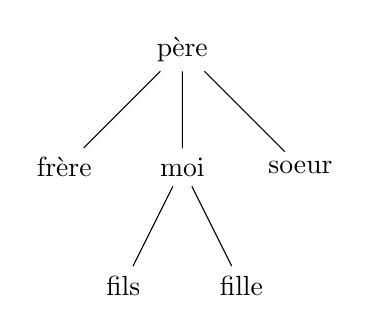
\begin{tikzpicture}[baseline=0pt]
 \node {père}
 child {node {frère}}
 child {node {moi}
 child {node {fils}}
 child {node {fille}}}
 child {node{soeur}};
 \end{tikzpicture} 
 & 
 \parbox[t]{8cm}{ 
  \BS{begin}\AC{tikzpicture} \\
  \BS{node} \AC{père} \\
  {\color{red}child} \AC{node \AC{frère}} \\
  {\color{red}child} \AC{node \AC{moi}\\
   {\color{red}child} \AC{node \AC{fils}}\\
   {\color{red}child} \AC{node \AC{fille}}}\\
  {\color{red}child} \AC{node\AC{soeur}};\\
  \BS{end}\AC{tikzpicture}\\
  } 
 \\  \hline  
 
 \end{tabular}

\bigskip
\begin{tabular}{|c|} \hline  
  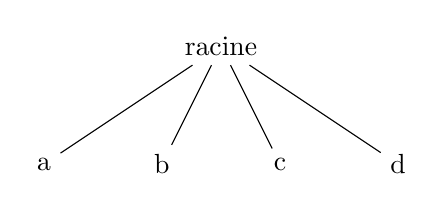
\begin{tikzpicture}[baseline=0pt]
\node {racine} child  foreach \name in {a,b,c,d} {node {\name}}; 
 \end{tikzpicture} 
\\  \hline  
\BS{node} \AC{racine} child  \RDD{foreach} \BS{name} in \AC{a,b,c,d} \AC{node \AC{\BS{name}}};
\\ \hline 
\end{tabular}  

 
  
\subsection{Orientation}

\begin{tabular}{|c|c|c|} \hline  
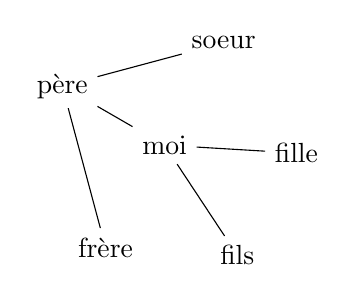
\begin{tikzpicture} 
  \node {père}[grow=-30] % angle
   child {node {frère}}
   child {node {moi}
   child {node {fils}}
   child {node {fille}}}
   child {node{soeur}};
   \end{tikzpicture}
&  
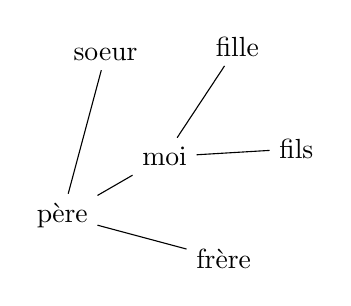
\begin{tikzpicture} 
  \node {père}[grow=30] % angle
   child {node {frère}}
   child {node {moi}
   child {node {fils}}
   child {node {fille}}}
   child {node{soeur}};
   \end{tikzpicture}
&  
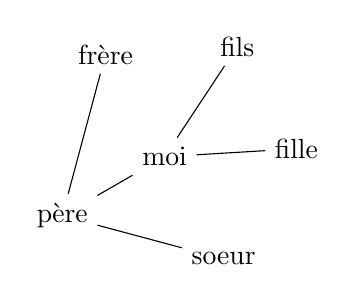
\begin{tikzpicture} 
  \node {père}[grow'=30] % angle
   child {node {frère}}
   child {node {moi}
   child {node {fils}}
   child {node {fille}}}
   child {node{soeur}};
   \end{tikzpicture}
\\ \hline 
\BS{node} \AC{père}[\RDD{grow=-30}]
&  
\BS{node} \AC{père}[\RDD{grow=30}]
&  
\BS{node} \AC{père}[\RDD{grow'}=30]
\\ \hline 
\end{tabular}
\bigskip  


\begin{tabular}{|c|c|c|} \hline  
 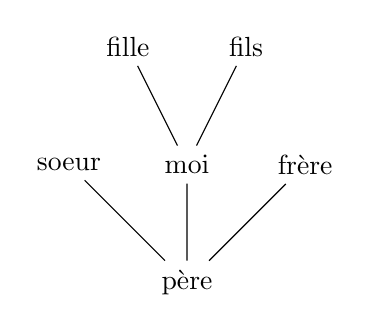
\begin{tikzpicture}
 \node {père}[grow=up]
 child {node {frère}}
 child {node {moi}
 child {node {fils}}
 child {node {fille}}}
 child {node{soeur}};
 \end{tikzpicture}
&  
  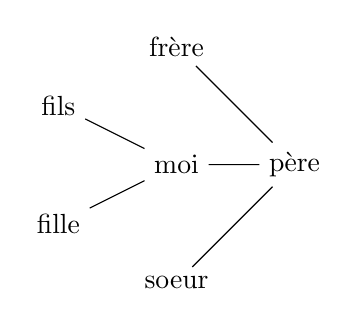
\begin{tikzpicture}
  \node {père}[grow=left]
  child {node {frère}}
  child {node {moi}
  child {node {fils}}
  child {node {fille}}}
  child {node{soeur}};
  \end{tikzpicture}
&  
 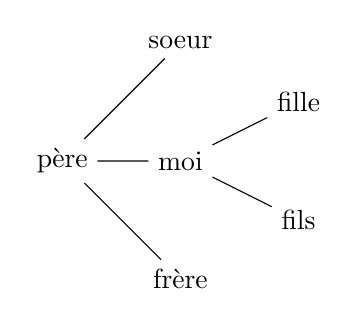
\begin{tikzpicture}
 \node {père}[grow=right]
 child {node {frère}}
 child {node {moi}
 child {node {fils}}
 child {node {fille}}}
 child {node{soeur}};
 \end{tikzpicture} 
\\ \hline  
\BS{node} \AC{père}[\RDD{grow=up}]
&  
\BS{node} \AC{père}[\RDD{grow=left}]
&  
\BS{node} \AC{père}[\RDD{grow=right}]
\\ \hline 
 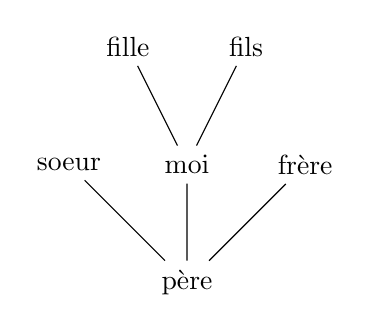
\begin{tikzpicture}
 \node {père}[grow=north]
 child {node {frère}}
 child {node {moi}
 child {node {fils}}
 child {node {fille}}}
 child {node{soeur}};
 \end{tikzpicture}
&  
  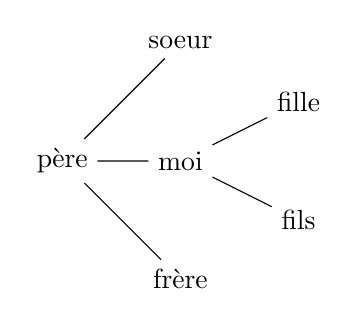
\begin{tikzpicture}
  \node {père}[grow=east]
  child {node {frère}}
  child {node {moi}
  child {node {fils}}
  child {node {fille}}}
  child {node{soeur}};
  \end{tikzpicture}
&  
 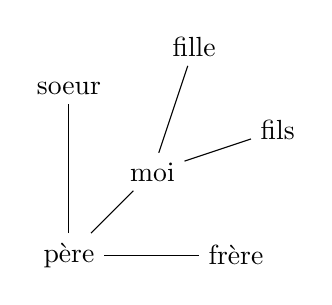
\begin{tikzpicture}
 \node {père}[grow=north east]
 child {node {frère}}
 child {node {moi}
 child {node {fils}}
 child {node {fille}}}
 child {node{soeur}};
 \end{tikzpicture} 
\\ \hline  
\BS{node} \AC{père}[\RDD{grow=north}]
&  
\BS{node} \AC{père}[\RDD{grow=east}]
&  
\BS{node} \AC{père}[\RDD{grow=north east}]
\\ \hline
\end{tabular}  

\bigskip 

\begin{tabular}{|c|c|} \hline  
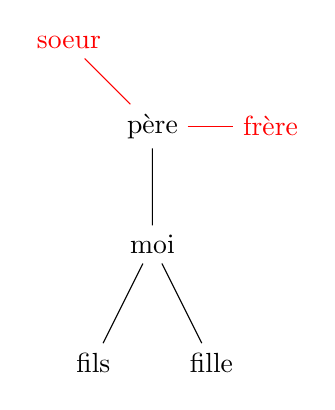
\begin{tikzpicture} [baseline=0pt]
  \node {père}
   child[grow=right,red] {node {frère}}
   child {node {moi}
   child {node {fils}}
   child {node {fille}}}
   child[grow=north west,red] {node{soeur}};
   \end{tikzpicture}
& 
\parbox[c]{8cm}{ 
  \BS{node} \AC{père}\\
   child[\RDD{grow=right},red] \AC{node \AC{frère}}\\
   child \AC{node \AC{moi}\\
   child \AC{node \AC{fils}}\\
   child \AC{node \AC{fille}}}\\
   child[\RDD{grow=north west},red] \AC{node\AC{soeur}};\\
   }
\\ \hline 
\end{tabular} 
   
%\subsection{N\oe uds }


\subsection{Distance}
%\subsubsection{Distance père fils}
\SbSSCT{Distance père fils}{Parent-child distance}

\begin{tabular}{|c|c|} \hline  
   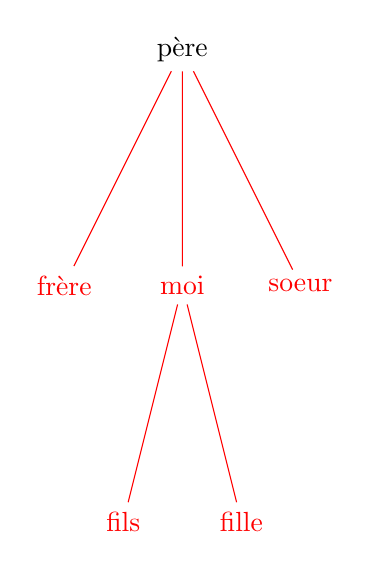
\begin{tikzpicture}
   \node {père}[level distance=3cm,red]
   child {node {frère}}
   child {node {moi}
   child {node {fils}}
   child {node {fille}}}
   child {node{soeur}};
   \end{tikzpicture}
&  
    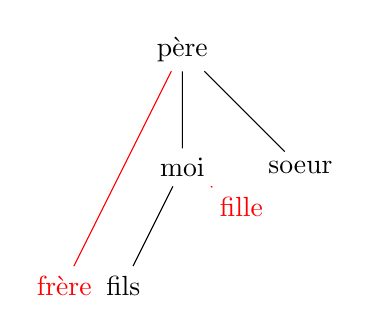
\begin{tikzpicture}
    \node {père}
    child[level distance=3cm,red] {node {frère}}
    child {node {moi}
    child {node {fils}}
    child[level distance=.5cm,red] {node {fille}}}
    child {node{soeur}};
    \end{tikzpicture} 
\\ \hline  
\BS{node} \AC{père}[level distance=3cm,red]
&  
child[level distance=3cm,red] \AC{node \AC{frère}}
\\
&  
child[level distance=.5cm,red] \AC{node \AC{fille}}
\\ \hline 
\multicolumn{2}{|c|}{\dft{} : level distance=15 mm} 
\\ \hline
\end{tabular} 

\bigskip

\begin{tabular}{|c|c|}  \hline  
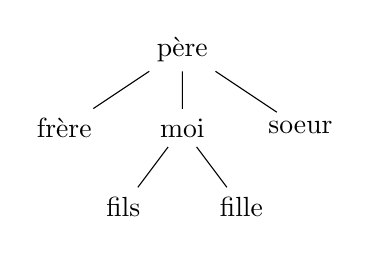
\begin{tikzpicture}
\node {père}[level 1/.style={level distance=1cm}]
child{node {frère}}
child {node {moi}
child {node {fils}}
child {node {fille}}}
child {node{soeur}};
\end{tikzpicture}
&
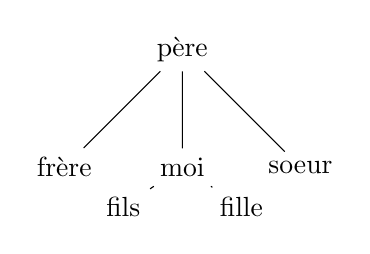
\begin{tikzpicture}
\node {père}[level 2/.style={level distance=.5cm}]
child{node {frère}}
child {node {moi}
child {node {fils}}
child {node {fille}}}
child {node{soeur}};
\end{tikzpicture}
 \\  \hline  
\BS{node} \AC{père}[\RDD{level 1/.style}=\AC{level distance=1cm}]
 &  
\BS{node} \AC{père}[\RDD{level 2/.style}=\AC{level distance=.5cm}]
 \\  \hline 
 \end{tabular} 

%\subsubsection{Distance frère soeur}
\SbSSCT{Distance père fils}{Two children distance}
    
 \begin{tabular}{|c|c|}  \hline  
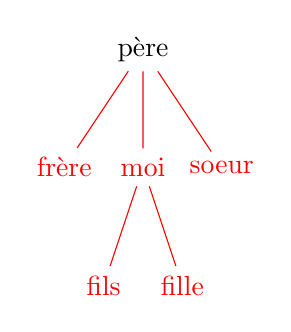
\begin{tikzpicture} 
  \node {père}[sibling distance=1cm,red]
   child {node {frère}}
   child {node {moi}
   child {node {fils}}
   child {node {fille}}}
   child {node{soeur}};
   \end{tikzpicture} 
 &  
 \begin{tikzpicture} 
   \node {père}[sibling distance=3cm,red]
    child {node {frère}}
    child {node {moi}
    child {node {fils}}
    child {node {fille}}}
    child {node{soeur}};
    \end{tikzpicture} 
 \\  \hline  
    \BS{node} \AC{père}[\RDD{sibling distance}=1cm,red]
 &  
   \BS{node} \AC{père}[\RDD{sibling distance}=3cm,red]
 \\  \hline 
 \multicolumn{2}{|c|}{\dft{} : sibling distance=15 mm} 
 \\ \hline
 \end{tabular} 

\bigskip
\begin{tabular}{|c|c|} \hline  
\TFRGB{Problème}{Problem} & solution 
\\ \hline 
 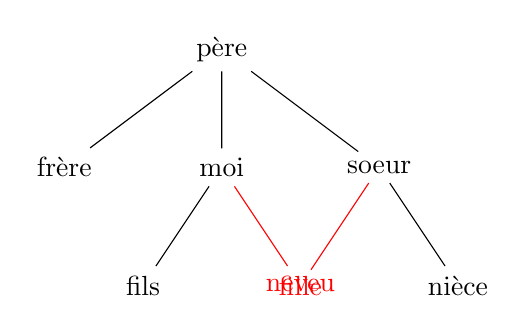
\begin{tikzpicture} 
   \node {père}[sibling distance=2cm]
    child {node {frère}}
    child {node {moi}
    child {node {fils}}
    child [red]{node {fille}}}
    child {node{soeur}
    child [red]{node {neveu}}
    child {node {nièce}}
    };
    \end{tikzpicture}
&  
 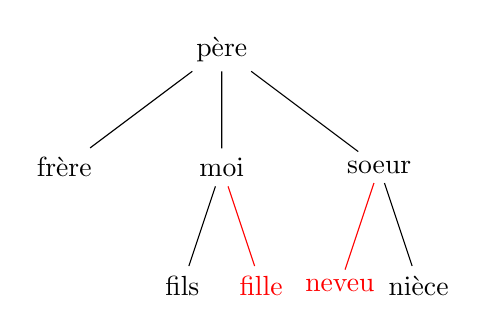
\begin{tikzpicture} 
   \node {père}[level 1/.style={sibling distance=2cm},
   level 2/.style={sibling distance=1cm}]
    child {node {frère}}
    child {node {moi}
    child {node {fils}}
    child  [red]{node {fille}}}
    child {node{soeur}
    child  [red]{node {neveu}}
    child {node {nièce}}
    };
    \end{tikzpicture}
\\ \hline  
[sibling distance=2cm]
&  
[level 1/.style={sibling distance=2cm},\\
&
   level 2/.style={sibling distance=1cm}]
\\ \hline 
\end{tabular} 
%
%--------------------------------------------------
%\subsection{Personnalisation des noeuds}
\SbSSCT{Personnalisation des noeuds}{Nodes customization}
  
  \begin{tabular}{|c|c|}   \hline

   \begin{tikzpicture}[baseline=0pt]
   \node[starburst,draw] {père}[grow=right]
   child {node[diamond,draw] {frère}}
   child {node[diamond,draw] {moi}
   child {node[ellipse,draw] {fils}}
   child {node[ellipse,draw] {fille}}}
   child {node[diamond,draw] {soeur}};
   \end{tikzpicture}
  &
   \parbox{8cm}{   
    \BS{node}[\RDD{starburst} \footnotemark[1] ,draw] \AC{père}[grow=right]\\ \\
    child \AC{node[\RDD{diamond},draw] {frère}}\\
    child \AC{node[\RDD{diamond},draw] {moi}\\
    child \AC{node[\RDD{ellipse},draw] {fils}}\\
    child \AC{node[\RDD{ellipse},draw] {fille}}}\\
    child \AC{node[\RDD{diamond},draw] {soeur}}; \\
    \\
 }
  \\   \hline 
    \begin{tikzpicture}[baseline=0pt,inner sep=4pt]
    \node[rectangle,double,draw,text width=1cm,text centered] {père et mère }[grow=right]
    child {node[red,ultra thick , draw,rotate=45] {frère}}
    child {node[blue,dashed, draw] {moi}
    child {node[ellipse,draw] {fils}}
    child {node[ellipse,fill] {fille}}}
    child {node[magenta,pattern=dots,draw] {soeur}};
    \end{tikzpicture} 
  &
    \parbox{10cm}{  
    \BS{node}[rectangle,double,draw,text width=1cm,text centered] \\ \AC{père}[grow=right,level distance=2cm]\\ \\
    child \AC{node{\color{red}[red,ultra thick,draw,rotate=45]} \AC{frère}}\\
    child \AC{node{\color{red}[blue,dashed, draw]} \AC{moi}\\
    child \AC{node{\color{red}[ellipse,draw]} \AC{fils}}\\
    child \AC{node {\color{red}[ellipse,fill]} \AC{fille}}}\\
    child \AC{node {\color{red}[magenta,pattern=dots,draw]} \AC{soeur}};\\
    }
  \\   \hline 
  \end{tabular} 
  
   \footnotetext[1]{ \TFRGB{autres types de n\oe uds voir}{Other types of nodes see} section \ref{ndbt} } 
%  
%%-----------------------------------------------


%\subsubsection{Nom des noeuds}
\SbSbSSCT{Nom des noeuds}{Nodes name}

\begin{tabular}{|c|c|} \hline  
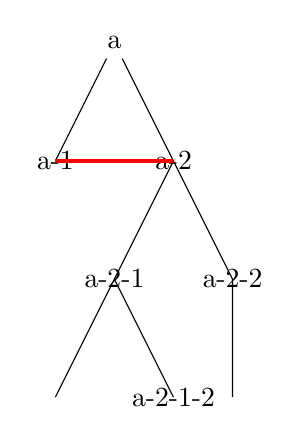
\begin{tikzpicture}[baseline=0pt]
\node (a) {a}
child
child {
child {child child}
child {child }
};
\node at (a-1) {a-1};
\node at (a-2) {a-2};
\node at (a-2-2) {a-2-2};
\node at (a-2-1) {a-2-1};
\node at (a-2-1-2) {a-2-1-2};
\draw[red,,ultra thick] (a-1) -- (a-2);
\end{tikzpicture}
& 

 \parbox[t]{8cm}{  
\BS{node} {\color{red}(a)} \AC{a}\\
child\\
child \AC{\\
child \AC{child child}\\
child \AC{child }\\
};\\
\BS{node} at {\color{red}(a-1)} \AC{a-1};\\
\BS{node} at {\color{red}(a-2)} \AC{a-2};\\
\BS{node} at {\color{red}(a-2-2)} \AC{a-2-2};\\
\BS{node} at {\color{red}(a-2-1)} \AC{a-2-1};\\
\BS{node} at {\color{red}(a-2-1-2)} \AC{a-2-1-2};\\
\\
\BS{draw}[red,ultra thick] {\color{red}(a-1)} -- {\color{red}(a-2)}; \\
}
%\BS{draw}[red,->] \AC(a-2-1-1) -- (a-1);
\\ \hline 
\end{tabular} 

\bigskip

\begin{tabular}{|c|c|} \hline  
\begin{tikzpicture}[baseline=0pt]
\node (a) {a}
child
child {
child {coordinate (b) child child}
child
};
\node at (a-1) {a-1};
\node at (a-2) {a-2};
\node at (b) {b};
\node at (a-2-2) {a-2-2};
\node at (b-1) {b-1};
\node at (a-2-1-2) {a-2-1-2};
\draw[red,,ultra thick] (a-1) -- (b-1);

\end{tikzpicture}
&  
\parbox[t]{8cm}{  
\BS{node}  (a) \AC{a} \\
child  \\
child { \\
child {coordinate (b) child child} \\
child \\
}; \\
\BS{node}  at (a-1) \AC{a-1}; \\
\BS{node}  at (a-2) \AC{a-2}; \\
\BS{node}  at {\color{red}(b)} \AC{b}; \\
\BS{node}  at (a-2-2) \AC{a-2-2}; \\
\BS{node}  at {\color{red}(b-1)} \AC{b-1}; \\
\BS{node}  at (a-2-1-2) \AC{a-2-1-2}; \\
\\
\BS{draw}[red,ultra thick] {\color{red}(a-1)} -- {\color{red}(b-1)}; \\
}
\\ \hline 
\end{tabular} 
 
%  %-------------------------------------
 


\bigskip

\begin{tabular}{|c|c|}\hline  
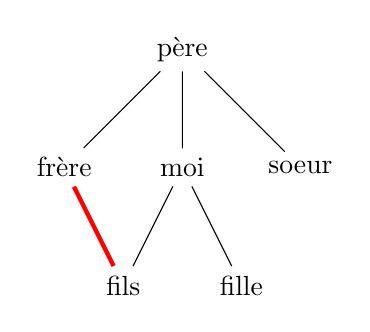
\begin{tikzpicture}
\node(a) {père}
child {node (b) {frère}}
child {node (c) {moi}
child {node (d) {fils}}
child {node (e) {fille}}}
child {node (f) {soeur}};
\draw[red,,ultra thick] (b) -- (d);
\end{tikzpicture}
& 
\parbox[b]{8cm}{

\BS{node} {\color{red}(a)} \AC{père}\\
child \AC{node {\color{red}(b)} \AC{frère}}\\
child \AC{node {\color{red}(c)} \AC{moi}\\
child \AC{node {\color{red}(d)} \AC{fils}}\\
child \AC{node {\color{red}(e)} \AC{fille}}}\\
child \AC{node {\color{red}(f)} \AC{soeur}};\\
\\
\BS{draw}[red,,ultra thick] {\color{red}(b)} -- {\color{red}(d)};\\
}
\\ \hline 
\end{tabular} 



 
%\subsubsection{Omission d'un noeud}
\SbSbSSCT{Omission d'un noeud}{Missing a node}

\begin{tabular}{|c|} \hline  
 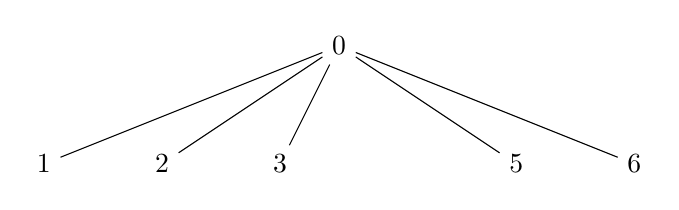
\begin{tikzpicture} %[level distance=10mm,sibling distance=5mm]
 \node {0} 
 child { node {1} }
 child { node {2} }
 child { node {3} }
 child[missing] { node {4} }
 child { node {5} }
 child { node {6} };
 \end{tikzpicture}
\\ \hline  
 child[\RDD{missing}] \AC{node \AC{4} }
\\ \hline 
\end{tabular} 

% \subsubsection{Modification du point d'accrochage}
\SbSbSSCT{Modification du point d'accrochage}{Attachment point modification}

 \begin{tabular}{|l|l|} \hline  
  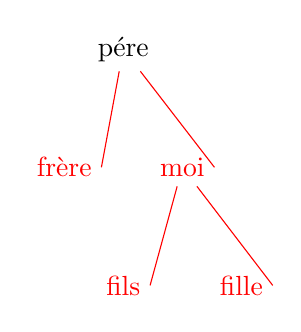
\begin{tikzpicture}
  \node {pére} [child anchor=east,red]
  child {node {frère}}
  child {node {moi}
  child  {node {fils}}
  child {node {fille} }
  };
  \end{tikzpicture}
 &  
  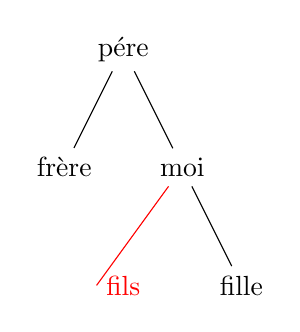
\begin{tikzpicture}
  \node {pére} 
  child {node {frère}}
  child {node {moi}
  child [child anchor=west,red] {node {fils}}
  child {node {fille} }
  };
  \end{tikzpicture}
 \\ \hline  
  \BS{node} \AC{pére} [{\color{red}child anchor=east},red]
 &  
  \BS{node} \AC{pére}
 \\ 
  child \AC{node \AC{frère}} &  child \AC{node \AC{frère}} \\
  child \{ node \AC{moi} &   child \{ node \AC{moi}\\
  child  \AC{node \AC{fils}} & child [\RDD{child anchor=west},red]  \AC{node \AC{fils}} \\
   child  \AC{node \AC{fils}} \}; & child  \AC{node \AC{fils}} \}; 
   \\  \hline 
 \end{tabular} 
\bigskip

\begin{tabular}{|l|l|} \hline  
 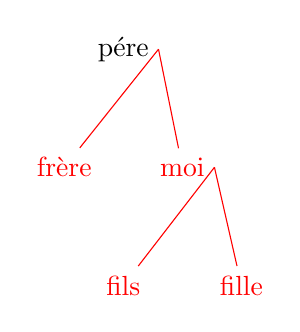
\begin{tikzpicture}
 \node {pére} [parent anchor=east,red]
 child {node {frère}}
 child {node {moi}
 child  {node {fils}}
 child {node {fille} }
 };
 \end{tikzpicture}
&  
 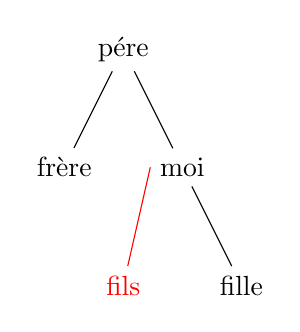
\begin{tikzpicture}
 \node {pére} 
 child {node {frère}}
 child {node {moi}
 child [parent anchor=west,red] {node {fils}}
 child {node {fille} }
 };
 \end{tikzpicture}
\\ \hline  
 \BS{node} \AC{pére} [\RDD{parent anchor=east},red]
&  
 \BS{node} \AC{pére}
\\ 
 child \AC{node \AC{frère}} &  child \AC{node \AC{frère}} \\
 child \{ node \AC{moi} &   child \{ node \AC{moi}\\
 child  \AC{node \AC{fils}} & child [\RDD{parent anchor=west},red]  \AC{node \AC{fils}} \\
  child  \AC{node \AC{fils}} \}; & child  \AC{node \AC{fils}} \}; \\
\hline 
\end{tabular} 

%------------------------------------------
%\subsection{Liaison}
\SbSbSSCT{Liaison}{Links}
%
\begin{tabular}{|c|c|c|} \hline  
 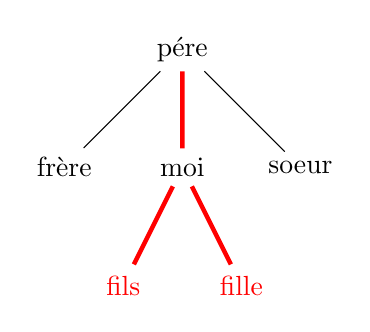
\begin{tikzpicture}
 \node {pére}  
child {node {frère}}
 child {node {moi}edge from parent[red,ultra thick]
 child  {node {fils}}
 child {node {fille} } }
 child {node{soeur}}; %;
 \end{tikzpicture}
&  
 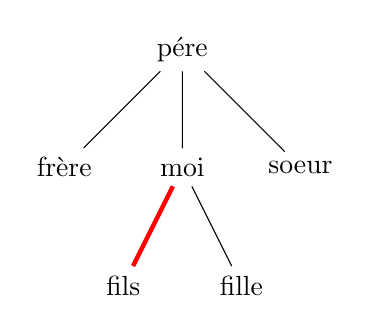
\begin{tikzpicture}
 \node {pére}
 child {node {frère}}
 child {node {moi} 
 child  {node {fils} edge from parent[red,ultra thick]}
 child {node {fille} } }
 child {node{soeur}};
 \end{tikzpicture}
&  
 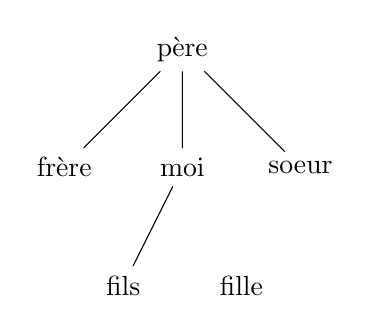
\begin{tikzpicture}
   \node {père} % angle
    child {node {frère}}
    child {node {moi}
    child {node {fils}}
    child {node {fille} edge from parent[draw=none]}}
    child {node{soeur}};
 \end{tikzpicture}
\\ \hline  

child \{node \AC{moi} &  child  \{node \AC{fils} & child \{ node \AC{fille} \\ 
\RDD{edge from parent}[red,ultra thick] & \RDD{edge from parent}[red,ultra thick] \} & \RDD{edge from parent}[draw=none] \} \\
\hline 
\end{tabular} 

\bigskip

 
\begin{tabular}{|c|} \hline  
 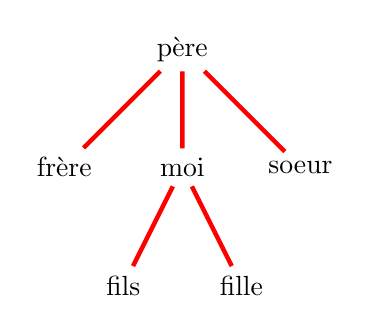
\begin{tikzpicture}
 [edge from parent/.style={draw,red,ultra thick}]
  \node {père} 
   child {node {frère}}
   child {node {moi}
   child {node {fils}}
   child {node {fille}}}
   child {node{soeur}};
 \end{tikzpicture}
\\ \hline  
 [\RDD{edge from parent/.style}=\AC{draw,red,ultra thick}] \\
 \BS{node} \AC{père} 
\\ \hline 
\end{tabular} 
 

 
%\subsubsection{\'Etiquetes sur liaisons}
\SbSbSSCT{\'Etiquetes sur liaisons}{Labels on link}

\begin{tabular}{|c|c|c|c|} \hline 
\multicolumn{4}{|c|}{\BS{node} \AC{père}
child \AC{node \AC{fils}  \RDD{edge from parent}
 node[left,red] \AC{texte}};} 
 \\ \hline
 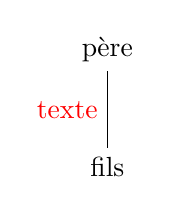
\begin{tikzpicture}
\node {père}
child {node {fils}  edge from parent
 node[left,red] {texte}};
 \end{tikzpicture}
&  
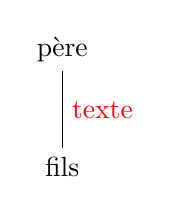
\begin{tikzpicture}
\node {père}
child {node {fils}  edge from parent
 node[right,red] {texte}};
 \end{tikzpicture}

&  
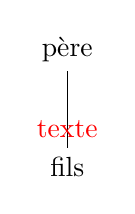
\begin{tikzpicture}
\node {père}
child {node {fils}  edge from parent
 node[near end,red] {texte}};
 \end{tikzpicture}
&  
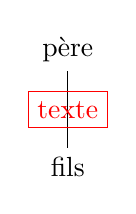
\begin{tikzpicture}
\node {père}
child {node {fils}  edge from parent
 node[draw,red] {texte}};
 \end{tikzpicture}
\\ \hline  
node[\RDD{left},red] & node[\RDD{right},red] & node[\RDD{near end},red] & node[\RDD{draw},red] \\ 
\hline 
\end{tabular} 








%\subsubsection{Personalisation des liaisons}
\SbSbSSCT{Personalisation des liaisons}{Links customization}
 
 \begin{tabular}{|c|c|c|}  \hline  
 \multicolumn{3}{|c|} { [ edge from parent path=
   \{(\BSS{tikzparentnode.south}) {\color{red}.. controls +(0,-1) and +(0,1) ..  }} \\
 \multicolumn{3}{|c|}{ (\BSS{tikzchildnode.north})\} ]}
 \\ \hline
  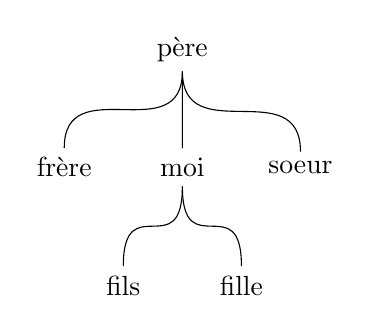
\begin{tikzpicture}[edge from parent path=
  {(\tikzparentnode.south) .. controls +(0,-1) and +(0,1)
  .. (\tikzchildnode.north)}]
 \node {père}
 child {node {frère}}
 child {node {moi}
 child {node {fils}}
 child {node {fille}}}
 child {node{soeur}};
  \end{tikzpicture}
 &  
 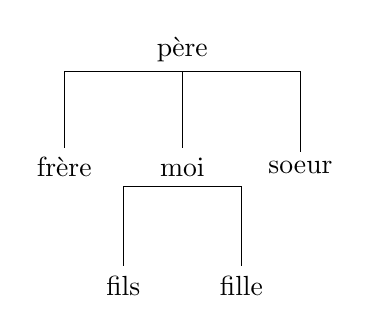
\begin{tikzpicture}[edge from parent path=
 {(\tikzparentnode.south) -|(\tikzchildnode.north)}]
 \node {père}
 child {node {frère}}
 child {node {moi}
 child {node {fils}}
 child {node {fille}}}
 child {node{soeur}};
 \end{tikzpicture}
&
 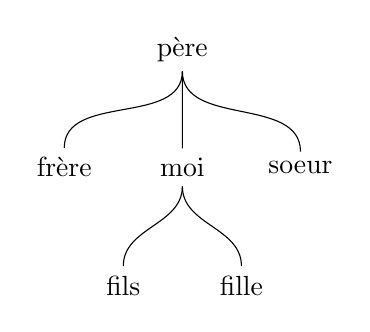
\begin{tikzpicture}[edge from parent path=
  {(\tikzparentnode.south) to[in=90,out=-90] (\tikzchildnode.north)}]
 \node {père}
 child {node {frère}}
 child {node {moi}
 child {node {fils}}
 child {node {fille}}}
 child {node{soeur}};
  \end{tikzpicture}     
 \\ \hline 
{\color{red} .. controls +(0,-1) and +(0,1)
  ..} &
{\color{red}-|} &  {\color{red}to[in=90,out=-90]}
  \\ \hline 
   \multicolumn{3}{|c|}{ \TFRGB{voir liaison de noeuds}{see links available : } section \ref{liaisons} }
   \\ \hline
 \end{tabular} 
 


%--------------------------------------------
\newpage
%\subsection{Options supplémentaires avec « library trees »}
\SbSSCT{Options supplémentaires avec « library trees »}{More options  with « library trees »}

\label{lib-trees}

%Insérer dans le préambule :

 \maboite{\BS{usetikzlibrary}\AC{trees}}
 
\begin{center}
\RRR{72}
\end{center}

%\subsubsection{Positions d'un fils et de  deux fils}
\SbSbSSCT{Positions d'un fils et de  deux fils}{One child and two childrenn position}

%\begin{tabular}{|c|c|c|} \hline  
%\begin{tikzpicture}
%[grow via three points={%
%one child at (0,0) and two children at (-.5,1) and (.5,1)}]
%\node at (0,0) {racine} child child child child;
%\draw[help lines] (-3,-1) grid (3,6); 
%\end{tikzpicture}
%&  
%\begin{tikzpicture}
%[grow via three points={%
%one child at (0,1) and two children at(-.5,1) and (.5,1)}]
%\node at (0,0) {racine} child child child child;
%\draw[help lines] (-3,-1) grid (3,6); 
%\end{tikzpicture}
%
%&  
%\begin{tikzpicture}
%[grow via three points={%
%one child at (0,-1) and two children at (-.5,1) and (.5,1)}]
%\node at (0,0) {racine} child child child child;
%\draw[help lines] (-3,-1) grid (3,6);
%\end{tikzpicture}
%\\ \hline  
%one child at (0,0)
%&  
%one child at (0,1)
%&  
%one child at (0,-1)
%\\ \hline 
%\end{tabular} 
%\bigskip
%
%\begin{tabular}{|c|c|c|} \hline  
%\begin{tikzpicture}[grow via three points={%
%one child at (0,0) and two children at (-.5,1) and (.5,1)}]
%\node at (0,-4.5) {racine} child child child child;
%\end{tikzpicture}
%&  
%\begin{tikzpicture}[grow via three points={%
%one child at (0,0) and two children at (0,1) and (1,1)}]
%\node at (0,-4.5) {racine} child child child child;
%\end{tikzpicture}
%&  
%\begin{tikzpicture}[grow via three points={%
%one child at (0,0)and two children at (-1,-.5) and (0,-.5)}]
%\node at (0,-4.5) {racine} child child child child;
%\end{tikzpicture}
%\\ \hline  
%at (-.5,1) and (.5,1)
%&  
%at (0,1) and (1,1)
%&  
%at (-1,-.5) and (0,-.5)
%\\ \hline 
%\end{tabular} 
%
%\bigskip

\begin{tabular}{|c|c|c|c|} \hline
\multicolumn{4}{|c|}{{\color{red}grow via three points}=\AC{
{\color{red} one child at} (0,1) {\color{red}and two children at} (-.5,1) {\color{red}and} (.5,1)} }  \\
\begin{tikzpicture}[red,ultra thick,grow via three points={%
one child at (0,1) and two children at (-.5,1) and (.5,1)}]
\node at (0,0) {un} child ;
\draw[help lines] (-1,-1) grid (1,2);
\end{tikzpicture}
&  
\begin{tikzpicture}[red,ultra thick,grow via three points={%
one child at (0,1) and two children at (-.5,1) and (.5,1)}]
\node at (0,0) {deux} child child;
\draw[help lines] (-1,-1) grid (1,2);
\end{tikzpicture}
&  
\begin{tikzpicture}[red,ultra thick,grow via three points={%
one child at (0,1) and two children at (-.5,1) and (.5,1)}]
\node at (0,0) {trois} child child child;
\draw[help lines] (-2,-1) grid (2,2);
\end{tikzpicture}
&  
\begin{tikzpicture}[red,ultra thick,grow via three points={%
one child at (0,1) and two children at (-.5,1) and (.5,1)}]
\node[] at (0,0) {quatre} child child child child;
\draw[help lines] (-2,-1) grid (2,2);
\end{tikzpicture}
\\ \hline  
&  &  &  \\ 
\hline 
\end{tabular} 

\bigskip

\begin{tabular}{|c|c|c|c|} \hline
\multicolumn{4}{|c|}{grow via three points=\AC{
one child at (0,1) and two children at {\color{red}(0,1)} and {\color{red}(1,1)}} }  \\ \hline
\begin{tikzpicture}[red,ultra thick,grow via three points={%
one child at (0,1) and two children at (0,1) and (1,1)}]
\node at (0,0) {un} child ;
\draw[help lines] (-1,-1) grid (1,2);
\end{tikzpicture}
&  
\begin{tikzpicture}[red,ultra thick,grow via three points={%
one child at (0,1) and two children at (0,1) and (1,1)}]
\node at (0,0) {deux} child child;
\draw[help lines] (-1,-1) grid (1,2);
\end{tikzpicture}
&  
\begin{tikzpicture}[red,ultra thick,grow via three points={%
one child at (0,1) and two children at (0,1) and (1,1)}]
\node at (0,0) {trois} child child child;
\draw[help lines] (-1,-1) grid (3,2);
\end{tikzpicture}
&  
\begin{tikzpicture}[red,ultra thick,grow via three points={%
one child at (0,1) and two children at (0,1) and (1,1)}]
\node[] at (0,0) {quatre} child child child child;
\draw[help lines] (-1,-1) grid (3,2);
\end{tikzpicture}
\\ \hline  
&  &  &  \\ 
\hline 
\end{tabular} 

\bigskip

\begin{tabular}{|c|c|c|c|} \hline
\multicolumn{4}{|c|}{grow via three points=\AC{
one child at (0,1) and two children at {\color{red}(-.5,1)} and {\color{red}(.5,1.5)}} }  \\  \hline  
\begin{tikzpicture}[red,ultra thick,grow via three points={%
one child at (0,1) and two children at (-.5,1) and (.5,1.5)}]
\node at (0,0) {un} child ;
\draw[help lines] (-1,-1) grid (1,3);
\end{tikzpicture}
&  
\begin{tikzpicture}[red,ultra thick,grow via three points={%
one child at (0,1) and two children at (-.5,1) and (.5,1.5)}]
\node at (0,0) {deux} child child;
\draw[help lines] (-1,-1) grid (1,3);
\end{tikzpicture}
&  
\begin{tikzpicture}[red,ultra thick,grow via three points={%
one child at (0,1) and two children at (-.5,1) and (.5,1.5)}]
\node at (0,0) {trois} child child child;
\draw[help lines] (-2,-1) grid (2,3);
\end{tikzpicture}
&  
\begin{tikzpicture}[red,ultra thick,grow via three points={%
one child at (0,1) and two children at (-.5,1) and (.5,1.5)}]
\node[] at (0,0) {quatre} child child child child;
\draw[help lines] (-2,-1) grid (2,3);
\end{tikzpicture}
\\ \hline  

\end{tabular} 
%
%\bigskip
%
%\begin{tabular}{|c|c|c|c|} \hline
%\multicolumn{4}{|c|}{grow via three points=\AC{
%one child at (0,1) and two children at (-.5,.5) and (.5,1)} }  \\
%\begin{tikzpicture}[red,ultra thick,grow via three 
%\end{tikzpicture}
%&  
%\begin{tikzpicture}[red,ultra thick,grow via three points={one child at (0,-.5) and two children at (-.5,.5) and (.5,1)} 
%\node at (0,0) {deux} child child;
%\draw[help lines] (-1,-1) grid (1,2);
%\end{tikzpicture}
%&  
%\begin{tikzpicture}[red,ultra thick,grow via three points={one child at (0,-.5) and two children at (-.5,.5) and (.5,1)}  
%\node at (0,0) {trois} child child child;
%\draw[help lines] (-1,-1) grid (3,2);
%\end{tikzpicture}
%%&  
%\begin{tikzpicture}[red,ultra thick,grow via three points={one child at (0,-.5) and two children at (-.5,.5) and (.5,1)}  
%\node[] at (0,0) {quatre} child child child child;
%\draw[help lines] (-1,-1) grid (3,2);
%\end{tikzpicture}
%\\ \hline  
%&  &  &  \\ 
%\hline 
%\end{tabular}
%
%\begin{tikzpicture}[grow via three points={%
%one child at (-1,-.5) and two children at (-1,-.5) and (0,-.75)}]
%\node at (0,0) {one} child;
%\node at (0,-1.5) {two} child child;
%\node at (0,-3) {three} child child child;
%\node at (0,-4.5) {four} child child child child;
%\end{tikzpicture}

%---------------------------------------

%\subsubsection{Liaison angulaire }
\SbSbSSCT{Liaison angulaire }{Angular linking}

\begin{tabular}{|c|c|c|} \hline  
\begin{tikzpicture}
[grow cyclic]
\node {racine} child child child child;
\end{tikzpicture}
&  
\begin{tikzpicture}
[grow cyclic,sibling angle=45]
\node {racine} child child child child;
\end{tikzpicture}
&  
\begin{tikzpicture}
[grow cyclic,sibling angle=90]
\node {racine} child child child child;
\end{tikzpicture}
\\ \hline  
[\RDD{grow cyclic}]
&  
[grow cyclic,\RDD{sibling angle}=45]
&  
[grow cyclic,\RDD{sibling angle}=90]
\\ \hline 
\end{tabular} 


\bigskip

%\begin{tabular}{|c|c|} \hline  
%\begin{tikzpicture}[baseline=0pt]
%[grow cyclic,level 1/.style={level distance=1cm,sibling angle=40},level 2/.style={level distance=5mm,sibling angle=20},level 3/.style={sibling angle=10}]
%\node {racine} child child  child {child child child }child child;
%\end{tikzpicture}
%& 
% \parbox[t]{8cm}{ 
%[grow cyclic,\\
%\RDD{level 1/.style}=\AC{sibling angle=40},\\
%\RDD{level 2/.style}=\AC{sibling angle=20}]\\
%\\
%\BS{node} \AC{racine} child \\
% child \\
% child \AC{child child child } \\
% 
% child \\
%  child;
%}
%\\ \hline 
%\end{tabular} 

%\bigskip
%
%\begin{tikzpicture}[baseline=0pt]
%[grow cyclic,
%level 1/.style={sibling angle=40},
%level 2/.style={sibling angle=10}]
%\node {racine} child child  {child child child child }child child;
%\end{tikzpicture}

%\bigskip
%\begin{tikzpicture}
%[grow cyclic,
%level 1/.style={level distance=8mm,sibling angle=60},
%level 2/.style={level distance=4mm,sibling angle=45},
%level 3/.style={level distance=2mm,sibling angle=30}]
%\coordinate [rotate=-90] % going down
%child foreach \x in {1,2,3}
%{child foreach \x in {1,2,3}
%{child foreach \x in {1,2,3}}};
%\end{tikzpicture}
%
%\begin{tikzpicture}
%[grow cyclic,
%level 1/.style={level distance=8mm},
%level 2/.style={level distance=4mm},
%level 3/.style={level distance=2mm}]
%\coordinate [rotate=-90] % going down
%child foreach \x in {1,2,3}
%{child foreach \x in {1,2,3}
%{child foreach \x in {1,2,3}}};
%\end{tikzpicture}
%
%
%\bigskip

\begin{tabular}{|c|c|} \hline  
\begin{tikzpicture}[baseline=0pt]
\node {root}
[clockwise from=30,sibling angle=30]
child {node {$30$}}
child {node {$0$}}
child {node {$-30$}}
child {node {$-60$}};
\end{tikzpicture}
&  
 \parbox[t]{8cm}{ 
\BS{node} \AC{racine}
[\RDD{clockwise from}=30,\RDD{sibling angle}=30] \\
\\
child \AC{node \AC{\$30\$} }\\
child \AC{node \AC{\$0\$} }\\
child \AC{node \AC{\$-30\$} }\\
child \AC{node \AC{\$-60\$ } };
}
\\ \hline 
\end{tabular} 

%-----------------------------------------------

%\subsubsection{Liaisons en fourchette}
\SbSbSSCT{Liaisons en fourchette}{Forking links}

\begin{tabular}{|c|c|} \hline  
\begin{tikzpicture}[baseline=0pt]
\node {père}
[edge from parent fork down]
child {node {frère}}
child {node {moi}
child[child anchor=north east] {node {fils}}
child {node {fille}}
};
\end{tikzpicture}
&  
\parbox[t]{9cm}{ 
\BS{node} \AC{père}
[\RDD{edge from parent fork down}] \\
\\
child \AC{node \AC{frère}} \\
child \AC{node \AC{moi} \\
child [child anchor=north east] \AC{node \AC{fils}} \\
child \AC{node \AC{fille}} \\
};
}
\\ \hline 
\end{tabular} 

\bigskip

\begin{tabular}{|c|c|} \hline  
\begin{tikzpicture}[baseline=0pt]
\node {père}
[edge from parent fork right]
child {node {frère}}
child {node {moi}
child {node {fils}}
child {node {fille}}
};
\end{tikzpicture}
&  
\parbox[t]{9cm}{ 
\BS{node} \AC{père} 
[\RDD{edge from parent fork right}] \\
\\
child \AC{node \AC{frère}} \\
child \AC{node \AC{moi} \\
child \AC{node \AC{fils}} \\
child \AC{node \AC{fille}} \\
};
}
\\ \hline 
\end{tabular} 

\bigskip

\begin{tabular}{|c|c|} \hline  
\begin{tikzpicture}[baseline=0pt]
\node {père}
[edge from parent fork right,grow=right]
child {node {frère}}
child {node {moi}
child {node {fils}}
child {node {fille}}
};
\end{tikzpicture}
&  
\parbox[t]{9cm}{ 
\BS{node} \AC{père} 
[edge from parent fork right,\RDD{grow=right}] \\
\\
child \AC{node \AC{frère}} \\
child \AC{node \AC{moi} \\
child \AC{node \AC{fils}} \\
child \AC{node \AC{fille}} \\
};
}
\\ \hline 
\end{tabular} 

  